\documentclass[border=6pt]{standalone}
\usepackage{tikz}
\usetikzlibrary{arrows.meta,positioning,calc,shapes.geometric,fit,backgrounds,patterns,matrix,decorations.pathreplacing}
\begin{document}
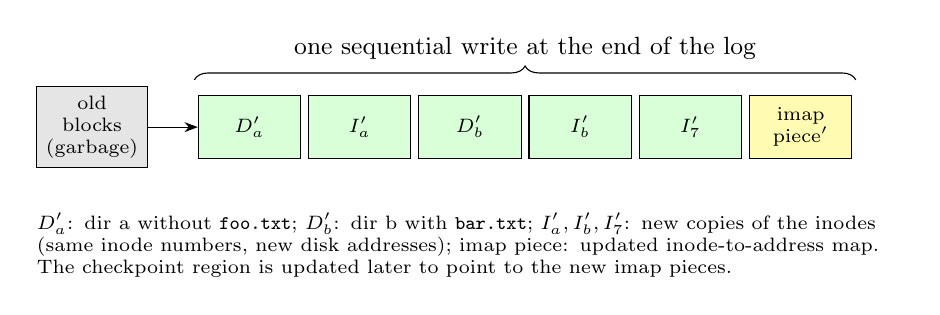
\begin{tikzpicture}[>=Stealth,font=\small]
\tikzstyle{blk}=[draw,minimum width=1.3cm,minimum height=0.8cm,align=center,font=\scriptsize]
\node[blk,fill=gray!20] (old) at (0,0) {old\\ blocks\\ (garbage)};
\node[blk,fill=green!15] (n1) at (2,0) {$D_a'$};
\node[blk,fill=green!15] (n2) at (3.4,0) {$I_a'$};
\node[blk,fill=green!15] (n3) at (4.8,0) {$D_b'$};
\node[blk,fill=green!15] (n4) at (6.2,0) {$I_b'$};
\node[blk,fill=green!15] (n5) at (7.6,0) {$I_7'$};
\node[blk,fill=yellow!30] (n6) at (9,0) {imap\\ piece$'$};
\draw[->] (old.east) -- (n1.west);
\draw[decorate,decoration={brace,amplitude=5pt}] (1.3,0.6) -- node[above=4pt,font=\small]{one sequential write at the end of the log} (9.7,0.6);
\node[font=\scriptsize,text width=11cm,align=left] at (4.8,-1.5) {$D_a'$: dir a without \texttt{foo.txt}; $D_b'$: dir b with \texttt{bar.txt}; $I_a', I_b', I_7'$: new copies of the inodes (same inode numbers, new disk addresses); imap piece: updated inode-to-address map. The checkpoint region is updated later to point to the new imap pieces.};
\end{tikzpicture}
\end{document}
